% GNUPLOT: LaTeX picture with Postscript
\begingroup
  \makeatletter
  \providecommand\color[2][]{%
    \GenericError{(gnuplot) \space\space\space\@spaces}{%
      Package color not loaded in conjunction with
      terminal option `colourtext'%
    }{See the gnuplot documentation for explanation.%
    }{Either use 'blacktext' in gnuplot or load the package
      color.sty in LaTeX.}%
    \renewcommand\color[2][]{}%
  }%
  \providecommand\includegraphics[2][]{%
    \GenericError{(gnuplot) \space\space\space\@spaces}{%
      Package graphicx or graphics not loaded%
    }{See the gnuplot documentation for explanation.%
    }{The gnuplot epslatex terminal needs graphicx.sty or graphics.sty.}%
    \renewcommand\includegraphics[2][]{}%
  }%
  \providecommand\rotatebox[2]{#2}%
  \@ifundefined{ifGPcolor}{%
    \newif\ifGPcolor
    \GPcolorfalse
  }{}%
  \@ifundefined{ifGPblacktext}{%
    \newif\ifGPblacktext
    \GPblacktexttrue
  }{}%
  % define a \g@addto@macro without @ in the name:
  \let\gplgaddtomacro\g@addto@macro
  % define empty templates for all commands taking text:
  \gdef\gplbacktext{}%
  \gdef\gplfronttext{}%
  \makeatother
  \ifGPblacktext
    % no textcolor at all
    \def\colorrgb#1{}%
    \def\colorgray#1{}%
  \else
    % gray or color?
    \ifGPcolor
      \def\colorrgb#1{\color[rgb]{#1}}%
      \def\colorgray#1{\color[gray]{#1}}%
      \expandafter\def\csname LTw\endcsname{\color{white}}%
      \expandafter\def\csname LTb\endcsname{\color{black}}%
      \expandafter\def\csname LTa\endcsname{\color{black}}%
      \expandafter\def\csname LT0\endcsname{\color[rgb]{1,0,0}}%
      \expandafter\def\csname LT1\endcsname{\color[rgb]{0,1,0}}%
      \expandafter\def\csname LT2\endcsname{\color[rgb]{0,0,1}}%
      \expandafter\def\csname LT3\endcsname{\color[rgb]{1,0,1}}%
      \expandafter\def\csname LT4\endcsname{\color[rgb]{0,1,1}}%
      \expandafter\def\csname LT5\endcsname{\color[rgb]{1,1,0}}%
      \expandafter\def\csname LT6\endcsname{\color[rgb]{0,0,0}}%
      \expandafter\def\csname LT7\endcsname{\color[rgb]{1,0.3,0}}%
      \expandafter\def\csname LT8\endcsname{\color[rgb]{0.5,0.5,0.5}}%
    \else
      % gray
      \def\colorrgb#1{\color{black}}%
      \def\colorgray#1{\color[gray]{#1}}%
      \expandafter\def\csname LTw\endcsname{\color{white}}%
      \expandafter\def\csname LTb\endcsname{\color{black}}%
      \expandafter\def\csname LTa\endcsname{\color{black}}%
      \expandafter\def\csname LT0\endcsname{\color{black}}%
      \expandafter\def\csname LT1\endcsname{\color{black}}%
      \expandafter\def\csname LT2\endcsname{\color{black}}%
      \expandafter\def\csname LT3\endcsname{\color{black}}%
      \expandafter\def\csname LT4\endcsname{\color{black}}%
      \expandafter\def\csname LT5\endcsname{\color{black}}%
      \expandafter\def\csname LT6\endcsname{\color{black}}%
      \expandafter\def\csname LT7\endcsname{\color{black}}%
      \expandafter\def\csname LT8\endcsname{\color{black}}%
    \fi
  \fi
    \setlength{\unitlength}{0.0500bp}%
    \ifx\gptboxheight\undefined%
      \newlength{\gptboxheight}%
      \newlength{\gptboxwidth}%
      \newsavebox{\gptboxtext}%
    \fi%
    \setlength{\fboxrule}{0.5pt}%
    \setlength{\fboxsep}{1pt}%
\begin{picture}(7200.00,5040.00)%
    \gplgaddtomacro\gplbacktext{%
      \csname LTb\endcsname%%
      \put(858,1993){\makebox(0,0)[r]{\strut{}$0.01$}}%
      \put(858,2464){\makebox(0,0)[r]{\strut{}$0.1$}}%
      \put(858,2935){\makebox(0,0)[r]{\strut{}$1$}}%
      \put(858,3406){\makebox(0,0)[r]{\strut{}$10$}}%
      \put(858,3877){\makebox(0,0)[r]{\strut{}$100$}}%
      \put(858,4348){\makebox(0,0)[r]{\strut{}$1000$}}%
      \put(858,4819){\makebox(0,0)[r]{\strut{}$10000$}}%
      \put(990,1641){\rotatebox{-45}{\makebox(0,0)[l]{\strut{}Terms:10-Runs:5000}}}%
      \put(1439,1641){\rotatebox{-45}{\makebox(0,0)[l]{\strut{}Terms:20-Runs:5000}}}%
      \put(1888,1641){\rotatebox{-45}{\makebox(0,0)[l]{\strut{}Terms:30-Runs:5000}}}%
      \put(2337,1641){\rotatebox{-45}{\makebox(0,0)[l]{\strut{}Terms:40-Runs:5000}}}%
      \put(2786,1641){\rotatebox{-45}{\makebox(0,0)[l]{\strut{}Terms:50-Runs:5000}}}%
      \put(3235,1641){\rotatebox{-45}{\makebox(0,0)[l]{\strut{}Terms:70-Runs:5000}}}%
      \put(3685,1641){\rotatebox{-45}{\makebox(0,0)[l]{\strut{}Terms:100-Runs:5000}}}%
      \put(4134,1641){\rotatebox{-45}{\makebox(0,0)[l]{\strut{}Terms:200-Runs:500}}}%
      \put(4583,1641){\rotatebox{-45}{\makebox(0,0)[l]{\strut{}Terms:500-Runs:500}}}%
      \put(5032,1641){\rotatebox{-45}{\makebox(0,0)[l]{\strut{}Terms:700-Runs:500}}}%
      \put(5481,1641){\rotatebox{-45}{\makebox(0,0)[l]{\strut{}Terms:1000-Runs:50}}}%
      \put(5930,1641){\rotatebox{-45}{\makebox(0,0)[l]{\strut{}Terms:3000-Runs:50}}}%
      \put(6379,1641){\rotatebox{-45}{\makebox(0,0)[l]{\strut{}Terms:5000-Runs:50}}}%
    }%
    \gplgaddtomacro\gplfronttext{%
      \csname LTb\endcsname%%
      \put(5392,4646){\makebox(0,0)[r]{\strut{}PI_}}%
      \csname LTb\endcsname%%
      \put(5392,4426){\makebox(0,0)[r]{\strut{}PITT}}%
      \csname LTb\endcsname%%
      \put(5392,4206){\makebox(0,0)[r]{\strut{}DN}}%
      \csname LTb\endcsname%%
      \put(5392,3986){\makebox(0,0)[r]{\strut{}TT_}}%
    }%
    \gplbacktext
    \put(0,0){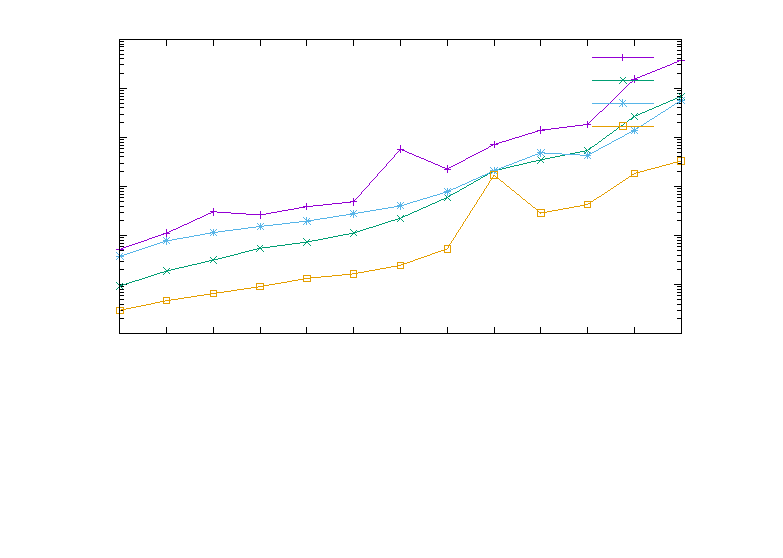
\includegraphics[width={360.00bp},height={252.00bp}]{graph1}}%
    \gplfronttext
  \end{picture}%
\endgroup
